\documentclass{article}
\usepackage[edges]{forest}
\usepackage{tikz}
\usetikzlibrary{positioning}


\title{Graph Theory - Travelling Salesman Problem using Brute Force Approach\\ \textit{Draft v0.1}}
\begin{document}
\maketitle

\textbf{1. Background - Pokémon Go Game}

In Pokémon Go, trainers can obtain essential items such as Poké Balls, potions, and other in-game resources by visiting designated locations called Poké Stops, where they can spin the stop's icon on their mobile device to receive a variety of items that aid in their Pokémon-catching adventures.

As a dedicated Pokémon Trainer, I would like to plan a journey to visit every Poké Stop near my school. The goal is to optimize the route for the shortest distance traveled while ensuring a return to my school.\\

\textbf{2. Problem Statement - Simple version}

As a Pokémon Trainer, I have identified three Poké Stops in my school's neighborhood, labeled as nodes 2, 3, and 4 (refer to Figure 1). Starting from my school (labeled as node 1), my objective is to find the shortest possible route that allows me to visit all three Poké Stops and return to my school.

\begin{figure}[h]
\centering
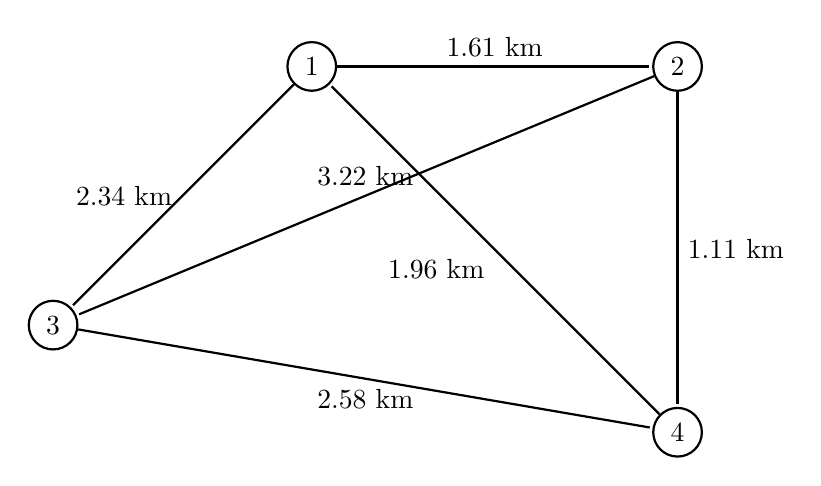
\begin{tikzpicture}[>=stealth,shorten >=1pt,auto,node distance=4cm,thick]

  \node[circle,draw] (1) {1};
  \node[circle,draw,right=of 1] (2) {2};
  \node[circle,draw,below left=of 1] (3) {3};
  \node[circle,draw,below=of 2] (4) {4};
  \path[-,draw] (1) edge node[above] {1.61 km} (2);
  \path[-,draw] (2) edge node[above] {3.22 km} (3);
  \path[-,draw] (3) edge node[below] {2.58 km} (4);
  \path[-,draw] (4) edge node[below left] {1.96 km} (1);
  \path[-,draw] (1) edge node[left] {2.34 km} (3);
  \path[-,draw] (2) edge node[right] {1.11 km} (4);

\end{tikzpicture}
\caption{Simple Pokémon Go Map with $3$ Poké Stops}
\textcolor{blue}{Above figure will be replaced by a real Pokémon Go Map - To Be Completed} 
\end{figure}

\textbf{3. Brute Force Approach}
\begin{enumerate}
    \item Represent nodes and paths in the matrix representation
    \item Generate all possible permutations using a tree representation
    \item Calculate total distance for each permutation for every branch of the tree
    \item Find the minimum distance  
\end{enumerate}

A matrix representation of a graph of 4 nodes and 6 paths
 \[
     \bordermatrix{ & node 1 & node 2 & node 3 & node 4\cr
       node 1 & 0 & 1.61 & 2.34 & 1.96\cr
       node 2 & 1.61 & 0 & 3.22 & 1.11\cr
       node 3 & 2.34 & 3.22 & 0 & 2.58\cr
       node 4 & 1.96 & 1.11 & 2.58 & 0} \qquad
 \]

A total of 6 permutations (branches) in a tree representation
\begin{figure}[h]
% \centering
\begin{forest}
  for tree={
    circle,
    draw,
    minimum size=1.5em,
    s sep=2em,
    l sep=2em,
  }
  [1
    [2, edge label={node[midway,above left] {1.61 km}}
      [3, edge label={node[midway,above left] {3.22 km}}
        [4, edge label={node[midway,above left] {2.58 km}}
          [1, edge label={node[midway,above left] {1.96 km}}, label=below:{\footnotesize sum=9.37 km}]
        ]
        [, phantom]
      ]
      [4, edge label={node[midway,above right] {1.11 km}}
        [, phantom]
        [3, edge label={node[midway,above left] {2.58 km}}
          [1, edge label={node[midway,above left] {2.34 km}}, label=below left:{\footnotesize sum=7.64 km}]
        ]
      ]
    ]
    [3, edge label={node[midway,above right] {2.34 km}}
      [2, edge label={node[midway,above left] {3.22 km}}
        [4, edge label={node[midway,above left] {1.11 km}}
          [1, edge label={node[midway,above right] {1.96 km}}, label=below:{\footnotesize sum=8.63 km}]
        ]
        [, phantom]
      ]
      [4, edge label={node[midway,above right] {2.58 km}}
        [, phantom]
        [2, edge label={node[midway,above left] {1.11 km}}
          [1, edge label={node[midway,above left] {1.61 km}}, label=below left:{\footnotesize sum=7.64 km}]
        ]
      ]
    ]
    [4, edge label={node[midway,above right] {1.96 km}}
      [2, edge label={node[midway,above left] {1.11 km}}
        [3, edge label={node[midway,above right] {3.22 km}}
          [1, edge label={node[midway,above right] {2.34 km}}, label=below:{\footnotesize sum=8.63 km}]
        ]
        [, phantom]
      ]
      [3, edge label={node[midway,above right] {2.58 km}}
        [, phantom]
        [2, edge label={node[midway,above right] {3.22 km}}
          [1, edge label={node[midway,above right] {1.61 km}}, label=below:{\footnotesize sum=9.37 km}]
        ]
      ]
    ]
  ]
\end{forest}
\caption{Brute Force Algorithm Analysis for Pokémon Go Routes}
\end{figure}

\textbf{4. Computation Costs}

If n presents the number of nodes, all possible permutations of node orderings is calculated as:
\[(n-1)!\]

For example, when $n = 4, 3! = 3 \times 2 \times 1 = 6$.\\\\\\\\\\

\textbf{5. Pros and Cons of Brute Force}

Pros
    \begin{enumerate}
        \item Simplicity: it is straightforward to implement, making them suitable for quick solutions and easy understanding.
        \item Guaranteed Solution: it guarantees finding the optimal solution, as it exhaustively explores all possibilities.
    \end{enumerate}

Cons
    \begin{enumerate}
        \item Inefficiency: it is highly inefficient, especially for large input sizes, as they examine all possible solutions without exploiting problem-specific
        \item Computational Complexity: The time and space complexity making it impractical. When $n=11$, there is $3,628,800 (10!)$ permutations. 
    \end{enumerate}

\textbf{6. Problem revisit - Complex Version}

\textcolor{blue}{Demonstrate a figure with a real Pokémon Go Map with $10$ Poké Stops - To Be Completed}\\


\textbf{7. Homework for audience}

TBC

\end{document}
